% n 边形内角和：以五边形为例，从 A1 引对角线分成 n-2=3 个三角形
\documentclass[tikz,border=4pt]{standalone}
\usepackage{ctex}
\usepackage{amsmath}
\usetikzlibrary{calc, angles, quotes, decorations.markings, arrows.meta}
\begin{document}
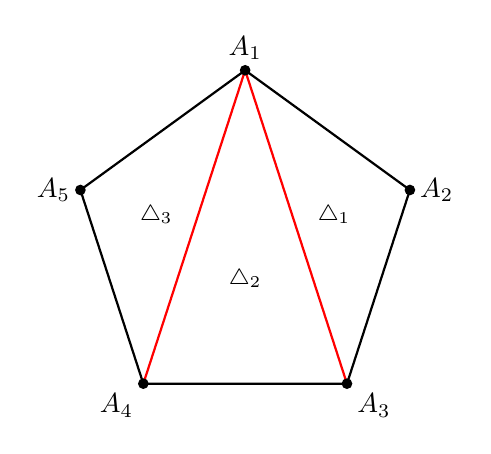
\begin{tikzpicture}[scale=1.0, thick]
  % 正五边形顶点（圆心在原点，半径 2.2，起始角 90°）
  \coordinate (A1) at (90:2.2);
  \coordinate (A2) at (18:2.2);
  \coordinate (A3) at (-54:2.2);
  \coordinate (A4) at (-126:2.2);
  \coordinate (A5) at (162:2.2);
  \draw (A1) -- (A2) -- (A3) -- (A4) -- (A5) -- cycle;
  % 从 A1 出发的两条对角线 → A3, A4
  \draw[red, thick] (A1) -- (A3);
  \draw[red, thick] (A1) -- (A4);
  % 三角形内部小角弧标注（仅意会，可省略）
  \foreach \pt in {A1,A2,A3,A4,A5} \filldraw (\pt) circle (1.5pt);
  \node[above]      at (A1) {$A_1$};
  \node[right]      at (A2) {$A_2$};
  \node[below right] at (A3) {$A_3$};
  \node[below left]  at (A4) {$A_4$};
  \node[left]       at (A5) {$A_5$};
  % 三角形标号
  \node[font=\footnotesize] at (barycentric cs:A1=1,A2=1,A3=1) {$\triangle_1$};
  \node[font=\footnotesize] at (barycentric cs:A1=1,A3=1,A4=1) {$\triangle_2$};
  \node[font=\footnotesize] at (barycentric cs:A1=1,A4=1,A5=1) {$\triangle_3$};
\end{tikzpicture}
\end{document}
